\chapter{Resultados e Discussões}

\section{Respostas das Juntas}
Para verificar se de fato são válidas as premissas assumidas na seção \ref{sec:controle_cinematico} para aplicação de uma estratégia de controle cinemático foi levantada para cada uma das juntas a resposta a uma onda quadrada tal que:
\[ u = A \sgn(\sin( 2\pi t/f)) \]
onde o período $T = 1/f = 1s$ e a amplitude $A = 0.5 rad/s$

\newlength{\imageheight}
\begin{figure}[!ht]
  \centering
  	\settoheight{\imageheight}{\includegraphics{./img/joints}}
    \includegraphics[width=\textwidth, clip=true, trim = 0 0.5\imageheight 0 0 0 mm]{./img/joints}
  \caption{Resposta das juntas}
\end{figure}


\section{Rastreamento de Trajetória}
A trajetória a ser rastreada é dada pelas equações:
\begin{gather}
\bm{x_d} = \m{75 \sin(\omega_n t) + \sin (4 \omega_n t) + 500 \\ 57 \\ 75 \cos(\omega_n t) + \cos(4\omega_n t) -67 \\ \omega_n \sin(\omega_nt) }
\qquad
\bm{\dot{x}_d} = \m{75\omega_n \cos(t\omega_n) + 300 \omega_n \cos(4t\omega_n) \\
0 \\
-75 \omega_n \sin(t \omega_n) - 300 \omega_n \sin(4t\omega_n) \\
\omega_n^2 \cos(t \omega_n)}
\end{gather}


\begin{figure}[!ht]
\centering
\begin{subfigure}{.5\textwidth}
  \centering
  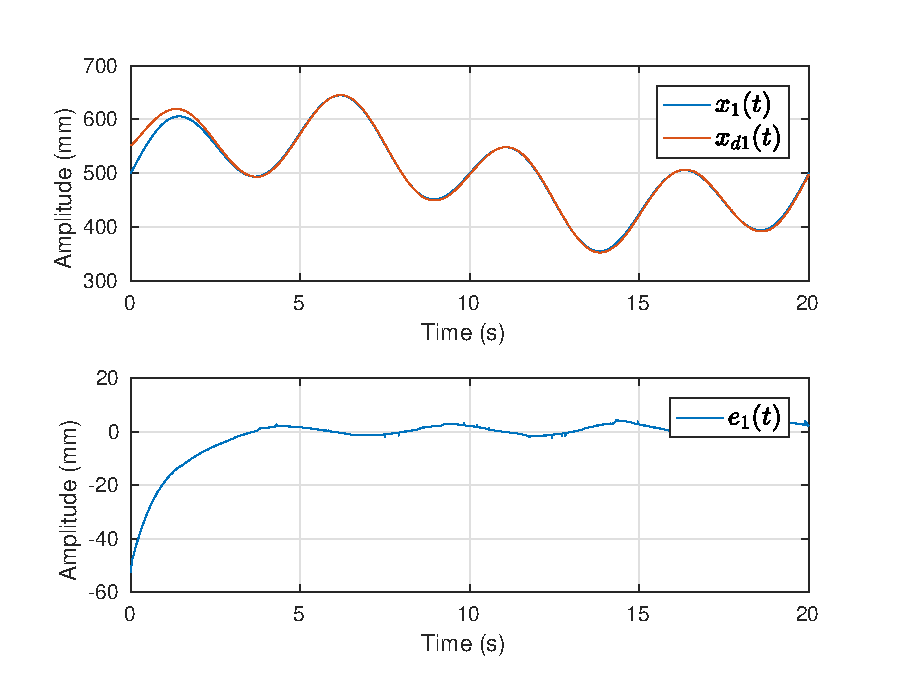
\includegraphics[width=\linewidth]{./img/trk1/x1.eps}
  \caption{$x_1$, $x_{d1}$ e $e_1$}
  \label{fig:sub1}
\end{subfigure}%
\begin{subfigure}{.5\textwidth}
  \centering
  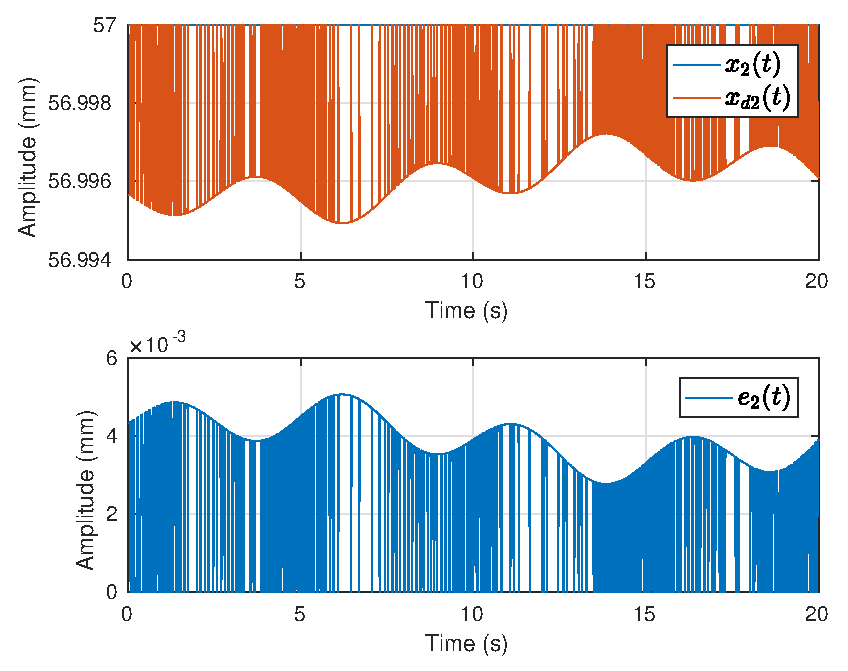
\includegraphics[width=\linewidth]{./img/trk1/x2.eps}
  \caption{$x_2$, $x_{d2}$ e $e_2$}
  \label{fig:sub2}
\end{subfigure}
\begin{subfigure}{.5\textwidth}
  \centering
  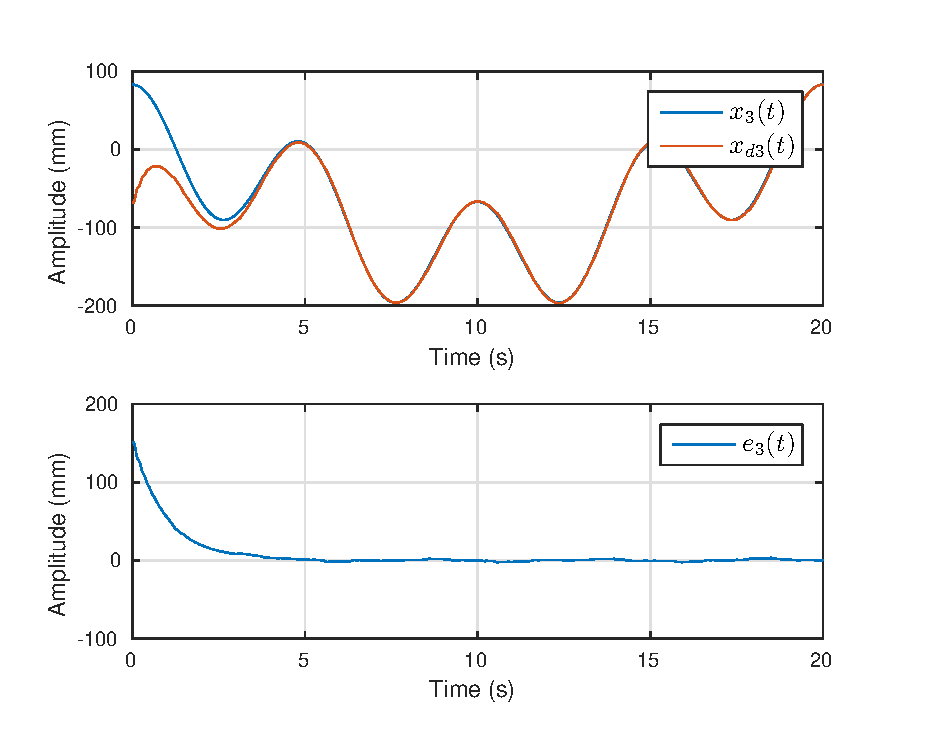
\includegraphics[width=\linewidth]{./img/trk1/x3.eps}
  \caption{$x_3$, $x_{d3}$ e $e_3$}
  \label{fig:sub1}
\end{subfigure}%
\begin{subfigure}{.5\textwidth}
  \centering
  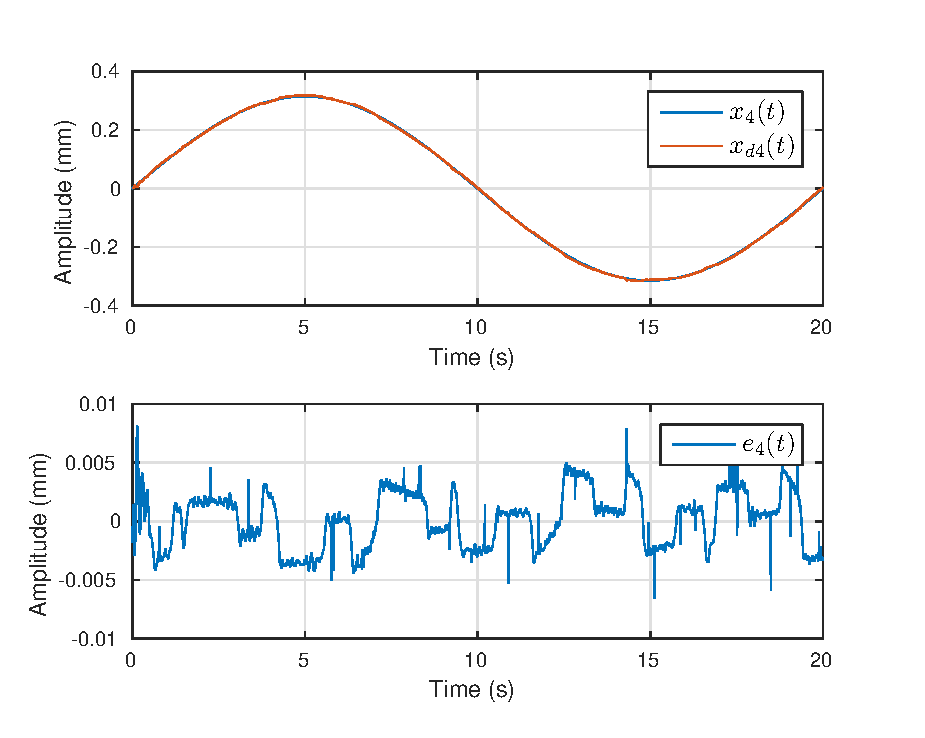
\includegraphics[width=\linewidth]{./img/trk1/x4.eps}
  \caption{$x_4$, $x_{d4}$ e $e_4$}
  \label{fig:sub2}
\end{subfigure}
\caption{A figure with two subfigures}
\label{fig:test}
\end{figure}

